% This is LLNCS.DEM the demonstration file of
% the LaTeX macro package from Springer-Verlag
% for Lecture Notes in Computer Science,
%
\documentclass{llncs}
\usepackage{graphicx} %package to manage images
\graphicspath{ {img/} }
\usepackage{makeidx}  % allows for indexgeneration
\usepackage{float}
\usepackage{caption}
\usepackage{subfig}
%
\begin{document}
%
\frontmatter          % for the preliminaries
%
\pagestyle{headings}  % switches on printing of running heads

\title{COMP5331 Final Report: \\ Implements and Applications of Toeplitz Inverse Covariance-Based Clustering}
\author{{\bf Group 13}: Guo Wenshuo, Cheung Tsz Him and Ding Mu Cong \\ (Implementaton Type Paper)}

\institute{The Hong Kong University of Science and Technology}

\maketitle % typeset the title of the contribution

\begin{abstract}

Time series clustering has shown its importance in providing useful information and applications in a wide range of research areas. Although a variety of clustering algorithms has been extensively explored, including the model-based clustering, density-based clustering and grid-based clustering, the difficulty in simultaneous segmentation and clustering, and the challenge in the interpretation of clustering results are remained. In this report, we investigated on the novel method designed by Dacid Hallac et al\cite{tiic} which offers an alternative for simultaneous segmentation and clustering on multi-variate time series data. We implemented and verified the superiority of TICC solver on two open-source real-world datasets, including the human activity time series data and gesture sensor time series data. We studied the results produced by TICC in detail and provide comparisons with the baseline methods: K-means and GMM. We also compared TICC with some deep learning classification model, i.e recurrent neural network (RNN) with long short-term memory (LSTM) cell when labels are present. Based on that, we analyzed the potential short-comings of TICC. We hope that our work could bring benefits on the further generalizations and applications of the TICC model, and offer insights for future research on time series clustering.

\end{abstract}

\section{Introduction}

Time series clustering has shown its significance in providing effective information and useful applications in many research fields, including economics \cite{DEMETRIADES1996387}, medicine \cite{DBLP:conf/smc/TsujinoO10}, bio-informatics \cite{DBLP:journals/bmcbi/WangJLZWWHZJXW17} and multimedia \cite{DBLP:conf/mue/NiennattrakulR07}. 

The central objective of clustering is to discover patterns in an unlabeled data set. Although different clustering algorithms have been extensively investigate, where the clustering algorithms objectively organizing data into homogeneous groups so that the within-group-object similarity is minimized and the between-group-object dissimilarity is maximized \cite{DBLP:journals/pr/Liao05}, the unique temple characteristics of time series data are the causes that fail most of conventional clustering techniques. For instance, for time series data with a high dimensionality, very high feature correlation, and large amount of noise, the clustering tasks have been regarded as an challenging research problem \cite{DBLP:journals/is/AghabozorgiST15}.

Multivariate time series take up the majority in real-world time series datasets. Sub-sequence clustering of these long time series could serve as a useful tool to discover repeated patterns in the data. The breaking down of the original time series into a sequence of states requires segmenting and clustering the multi-variate time series simultaneously, which is an interesting and difficult challenge. 

In this report, we specially investigated on the applications and improvements of Toeplitz Inverse Covariance-Based Clustering \cite{tiic}, which provides a novel way for simultaneous segmentation and clustering. We implemented TICC algorithm and tested it on two multi-variate time series data sets, the human activity data and gesture data. We then compared its performance with K-means and GMM and analyzed their prediction results in great details. Further more, We compared TICC with classification models like RNN using LSTM on these two labeled data sets, and revealed the short-comes of TICC is that It cannot handle frequent state transitions (or to say short latent sub-sequences equivalently). We also examined the effects of 4 hyper-parameters of TICC algorithm based ton the empirical study on human activity data. Based on these empirical summaries, we proposed our understanding on choosing the hyper-parameters.

\section{Previous Work}

Clustering problems are central to many data mining and knowledge discovery tasks. In this section, the literature review and discussions on some proposed papers on time series clustering and their applications are presented. 

In recent years, mining repeated patterns in temporal data has been shown to serve as a useful way to gain effective information from time series datasets. Mining the patterns from time series could help simplify the original complicated datasets into a temporal sequence of small clusters. However, the simultaneous segmentation and clustering and comprehensive understanding of the clustering results have remained to be current difficulties in the research area.

Traditional methods including K-means have been applied on the clustering of different time series data. Recent work has demonstrated the usefulness of time series representations to the raw multimedia data \cite{DBLP:conf/mue/NiennattrakulR07}, where k-medoids algorithm with Dynamic Time Warping (DTW) has been widely used.The Dynamic Time Warping could provide the ideal shape-based similarity measurement which can break the limitation of one-to-one mapping in the Euclidean distance metric. However, the K-means clustering may fail to provide correct results especially when Dynamic Time Warping (DTW) is used as the distance measure in averaging the shape of the time series. The potential causes and suggestions were discussed and presented by Vit Niennattarakul et al \cite{DBLP:conf/mue/NiennattrakulR07}. In 2003, \cite{xiong2004time}, an expectation-maximization(EM) algorithm for learning the mixing coefficients and the parameters of the component models was presented with interesting outcomes. The Bayesian information criterion was used to determine the number of clusters in the data. And results showed that the method compares favorably with other previous methods for similar time series clustering tasks. However, one remained problem is that for EM-based methods, the clustering performance could degrade significantly when the underlying clusters are close to each other. Therefore, possible extensions remain in need to improve the performance of EM-based clustering algorithms. 

\section{Implementation and Model Comparison}
\subsection{Data set}
The TICC algorithm is applied to 2 multivariate, time-series data sets, namely Human Activity Data set \cite{Stisen:2015:SDD:2809695.2809718} and Gesture Data set \cite{Madeo:2013:GUS:2480362.2480373} to evaluate its performance. 

\subsubsection{Human Activity Data set:}
The Human Activity Data set consists of the accelerometer and gyroscope readings in smart phones and smart watches of 9 users. The readings are recorded while users are performing 6 different activities: “Standing”, “Sitting”, “Biking”, Walking”, “Stairs Up” and “Stairs Down”. Each sensor generates 3 values in every time stamp, which are the xyz-axis reading from the sensors, forming altogether 6 features. The task is to cluster the 6 activities based on the sensor readings. Through observing the ground truth, the clusters are large in size, which means the same activity lasts for long period of time.

\subsubsection{Gesture Dataset}
The Gesture Data set contains the xyz-axis reading of left and right hands, head, spine and left and right wrists from the Microsoft Kinect sensor, forming altogether 18 features. The readings are recorded while users are demonstrating 5 different gestures: “Rest”, “Preparation”, “Stroke”, “Hold” and “Retraction”. The task is to cluster the 5 gestures based on the position readings. Different from the Human Activity Data set, the clusters are smaller, which means the gesture changes frequently throughout the time series.

\subsection{Data Pre-processing}
For the Human Activity Data set, we picked a fixed user (user id = a from the dataset) as our target subject and smartphone model nexus 4 as our sensor. The smartphone accelerometer and gyroscope readings with the same time stamps are joined. The timestamps, index and the data with missing labels are discarded. Among the total 600K data points from user A, we evenly sampled the time series into around 20K data points.  

For the Gesture Dataset, the entire dataset, around 10K data points, is used. Timestamps and missing data are dropped. 

\subsection{Implementation}
We adopted most code from the TICC solver.py provided by the original paper \cite{tiic} with slight modification on the input and output utilities. We also implemented the K-means clustering, Gaussian Mixture Model and some visualization utilities to benchmark, visualize and evaluate TICC performance. Apart from those classical clustering algorithms, when labels are present, it is also possible to classify the sequence segments by classification methods. We also implement a RNN model using LSTM cells and compared its accuracy with TICC. Although it is not a fair competition, since TICC is an unsupervised learning algorithm, it answers the question that why TICC is still preferable even when we have enough labels to train a deep neural network.

\subsection{Baseline Comparisons}
We compared the accuracy of the cluster assignments from TICC, K-Means Clustering and Gaussian Mixture model, with the ground truth labels. We also compared it with LSTM RNN and discussed their differences.

\subsection{Comparison on Human Activity Data}
We run TICC, K-means and GMM on the human activity data. From the results, as shown in Fig. 1, we can observe that clearly TICC did a better job compared to K-means and GMM. Since it is a subsequence clustering algorithm, TICC classify each subsequence a a whole, which greatly reduce the error. Based on the clustering results, we also generate the confusion matrix where we label each clusters so that the accuracy is maximized. From the confusion matrices, Fig. 2, we can see that TICC perfectly clustered the 6 classes of activities, with very slight messing up between the "Stairs Up" and "Standing" states. While K-means and GMM perform much more poorly. From Fig. 2b we found that K-means tends to classify many subsequences as "Sitting" and "Standing", although it got good accuracy on recognizing these two states, it also miss interpret many other activities as "Sitting" and "Standing". For GMM, "Standing", "Stairs down" and "Walking" are best recognized, with around $0.5$ accuracy. While "Sitting" is often misunderstand as "Standing".

\begin{figure}[H]
    \centering
    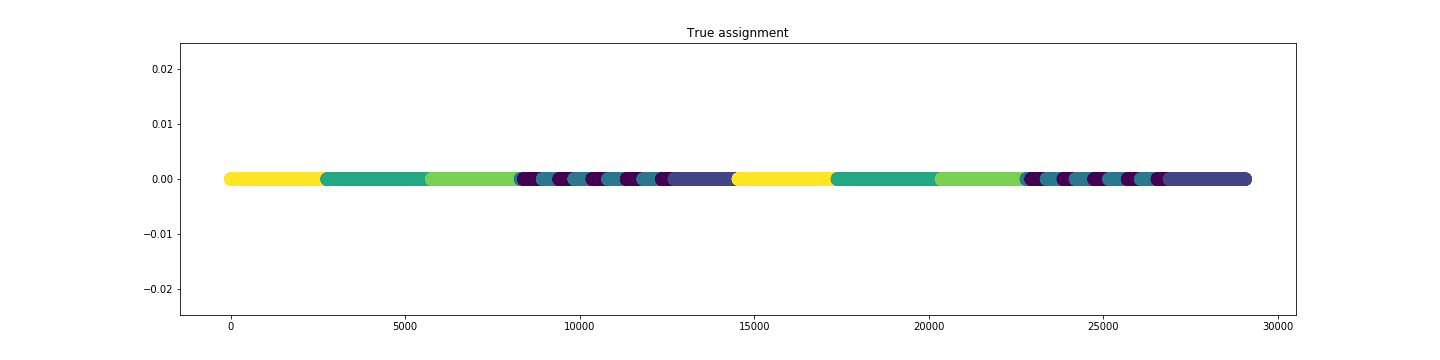
\includegraphics[width=.49\textwidth]{True.png}
    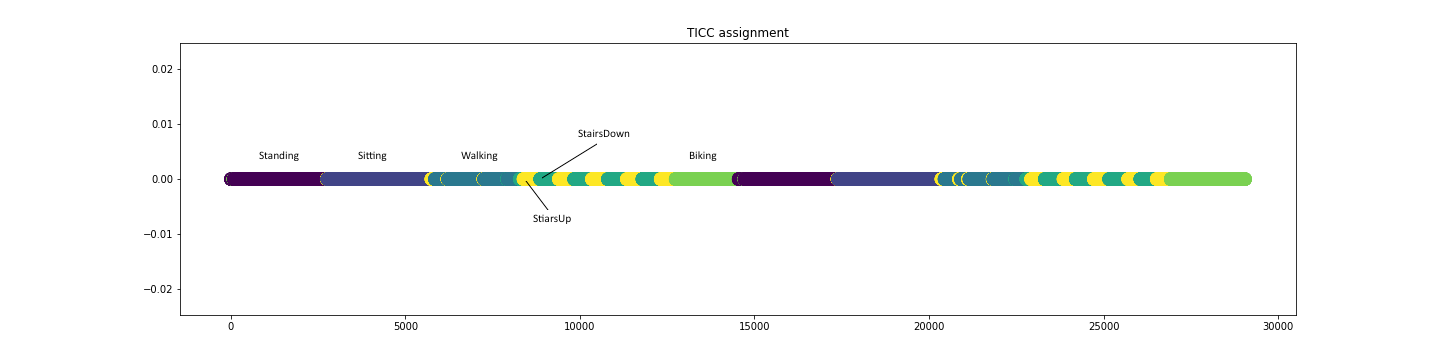
\includegraphics[width=.49\textwidth]{TICC.png}
    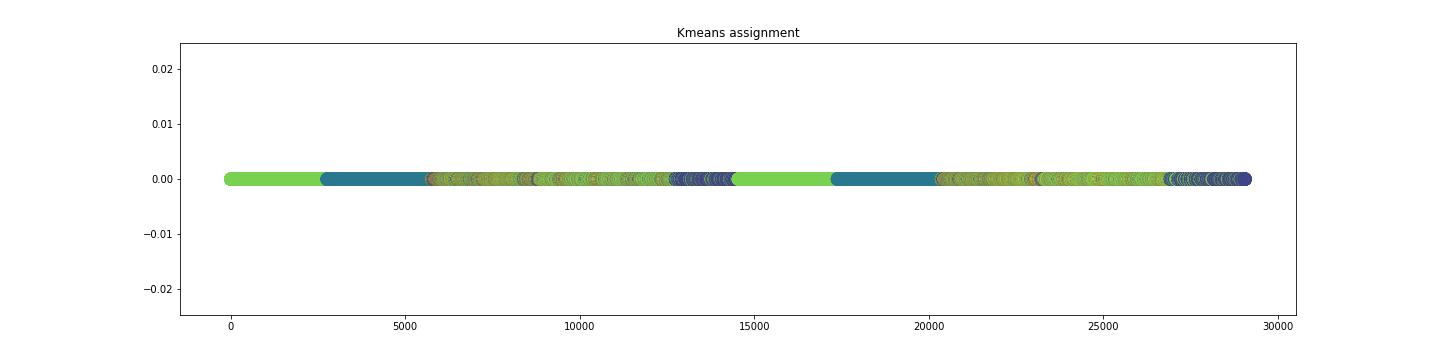
\includegraphics[width=.49\textwidth]{KMeans.png}
    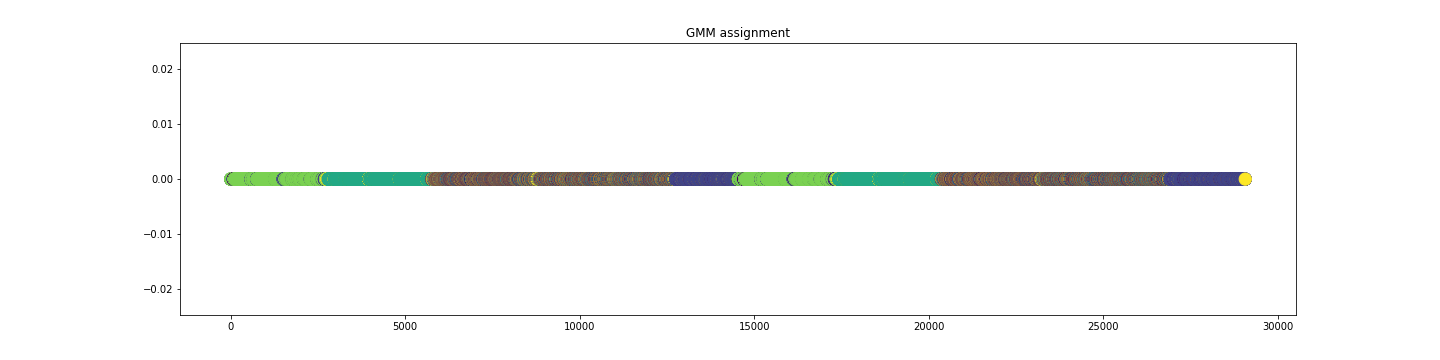
\includegraphics[width=.49\textwidth]{GMM.png}
    \caption{Human Activity Cluster assignment of (a) True Labels (b) TICC (c) KMeans (d) GMM. Each different color represent a unique label in the time series.}
    \label{fig:human}
\end{figure}

\begin{figure}[H]
	\centering
	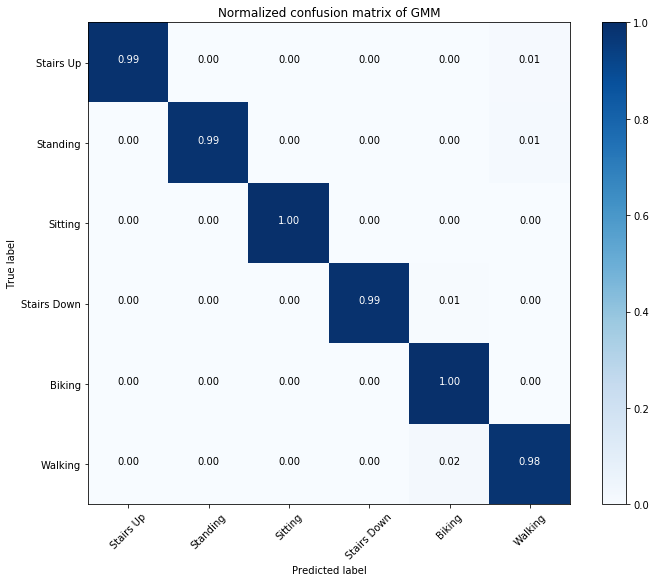
\includegraphics[width=.49\textwidth]{CFM_TICC.png}
	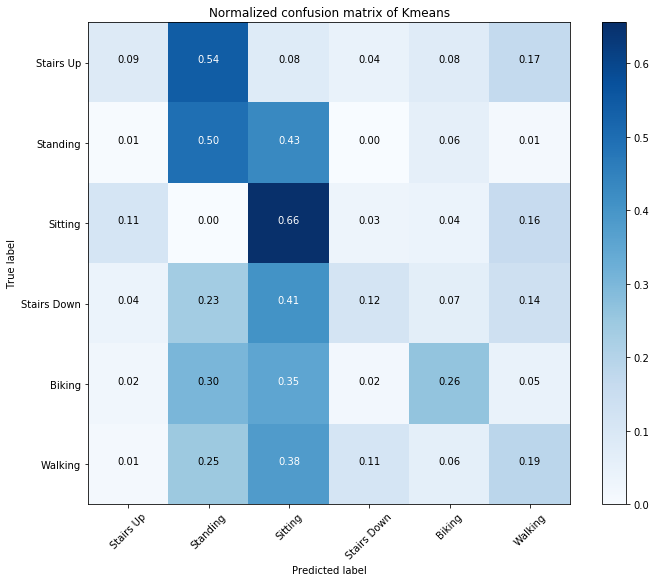
\includegraphics[width=.49\textwidth]{CFM_Kmeans.png}
	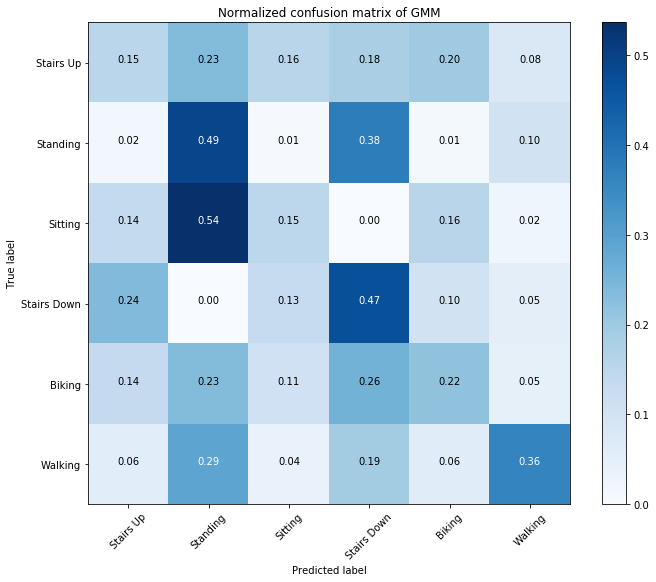
\includegraphics[width=.49\textwidth]{CFM_GMM.png}
	\caption{Human Activity Cluster assignment of (a) True Labels (b) TICC (c) KMeans (d) GMM. Each different color represent a unique label in the time series.}
	\label{fig:human_cfm}
\end{figure}

\subsection{Comparison on Gesture Data}
We found  that TICC, K-means and GMM clustered did not generate satisfactory results on the Gesture dataset. It is observed that the time series gesture changes frequently and each gesture lasts for a short period of time (Fig. 3a). However, even the TICC model is set to capture smaller window and use small smoothing penalty, which creates more segments, the model fails to cluster the gesture in the middle part (Fig. 3b). However, same as Human Data set, other benchmark models, like KMeans and GMM perform even worse (Table 1).
\begin{table}[H]
    \centering
    \begin{tabular}{l|c|c}{\bf Model} & \bf Accuracy on Human Dataset &\bf Accuracy on Gesture Dataset \\
    \hline
    TICC        & 92.88\%  & 14.21\%  \\
    KMeans      & 42.69\%  & 3.11\%   \\
    GMM         & 58.76\%  & 4.98\%   \\
 \end{tabular}
    \caption{Comparison between different models on two datasets}
    \label{tab:acc}
\end{table}

\begin{figure}[H]
    \centering
    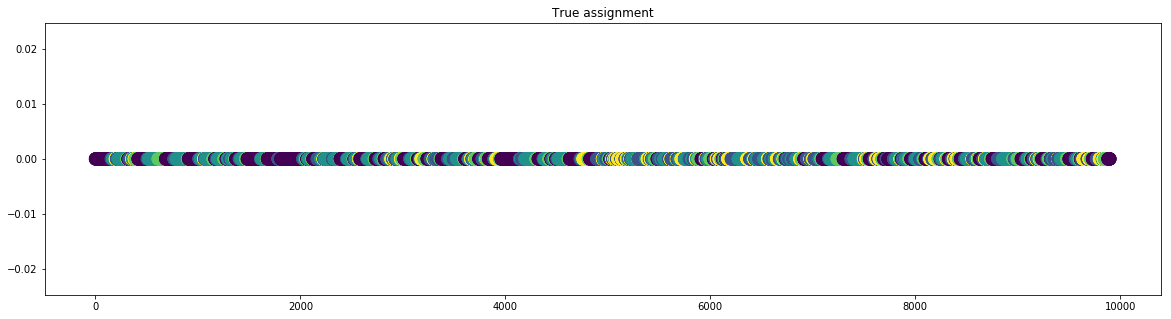
\includegraphics[width=0.49\textwidth]{TrueGestures.png}
    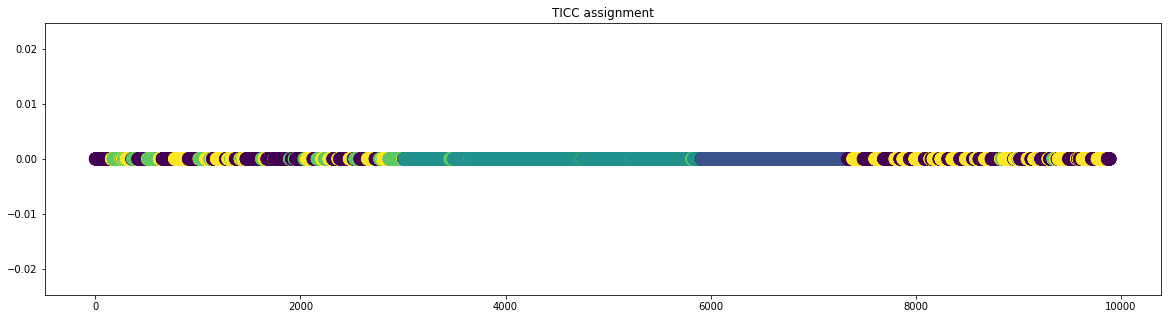
\includegraphics[width=0.49\textwidth]{TICC_gesture.png}
    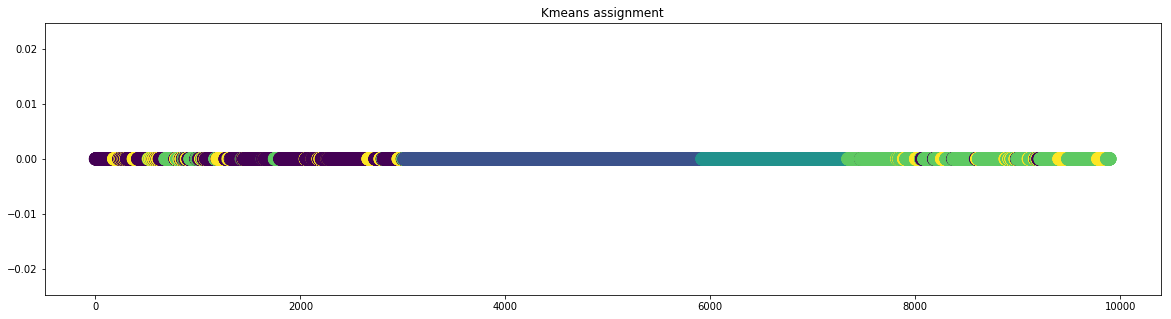
\includegraphics[width=0.49\textwidth]{Kmeans_gesture.png}
    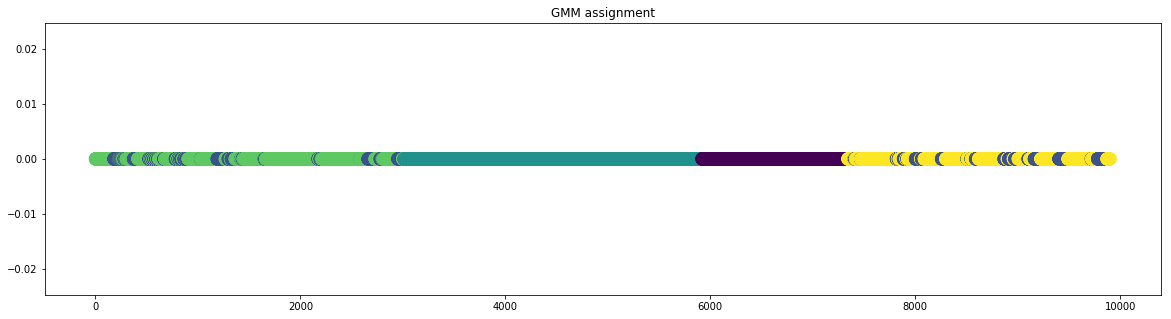
\includegraphics[width=0.49\textwidth]{GMMgesture.png}
    \caption{Gesture Cluster assignment of (a) True Labels (b) TICC (c) KMeans (d) GMM}
    \label{fig:gesture}
\end{figure}

\subsection{Comparison with RNN using LSTM}
It is an interesting question that whether TICC could event beat some successful classification models using recurrent neural networks (RNNs) and long short-term memory cells (LSTM cells), even though TICC does not require the labels. Compared to RNN classification model, TICC is intrinsically an unsupervised learning method which preserves the inner consistency of sub-sequences. This feature is very valuable compared to other sequence-to-sequence learning approaches since many real word data maintains this sub-sequence consistency, e.g. our human activity and gesture data. In this subsection, we compare TICC with LSTM RNN and discuss their pros and cons.

We first trained a simple LSTM network on the gesture data. Since it is one long sequence, we split it into around 1K short sequences of length $25$ before feed into the network. This splitting may already destroy the latent sub-sequence structure, but since it is unknown to us, we cannot do better. The input tensor is of shape (number of sequences, number of time units, number of features (sensor variables)), while the output shape is (number of sequences, number of time units, number of classes). We use softmax function at the output layer and cross entropy as loss function. The network structure is generally as shown in Fig. 4.

\begin{figure}[H]
	\centering
	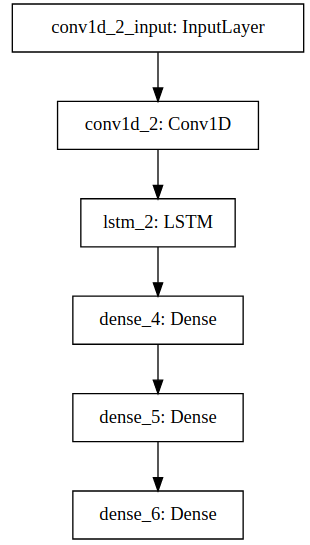
\includegraphics[width=0.2\textwidth]{NetworkStructure.png}
	\caption{Structure of LSTM RNN for comparison}
	\label{fig:network}
\end{figure}

Where the LSTM layer is put in between of convolution 1D layer and a block of 3 dense (fully-connected) layers. The 1D convolution layer (CNN) could effectively select representations along the time axis. While LSTM are capable to handle relatively long sequence inputs. The dense layers are merely for generating the predictions. We carefully tuned the hyper-parameters of this LSTM RNN and test it on the human activity data. The learning curve are shown in Fig. 5 as follows,

\begin{figure}[H]
	\centering
	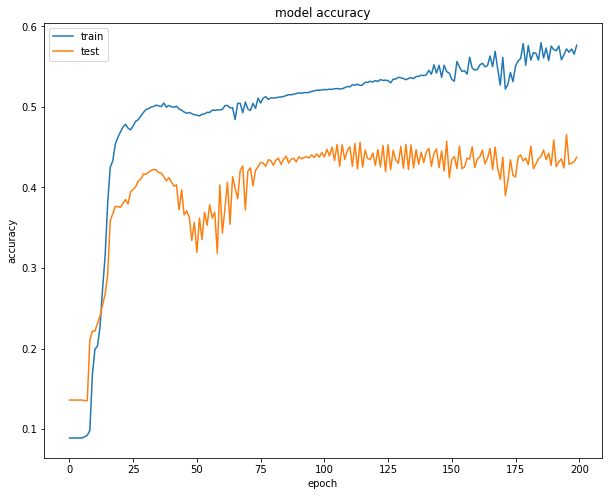
\includegraphics[width=0.45\textwidth]{LSTM_Accuracy_GD.png}
	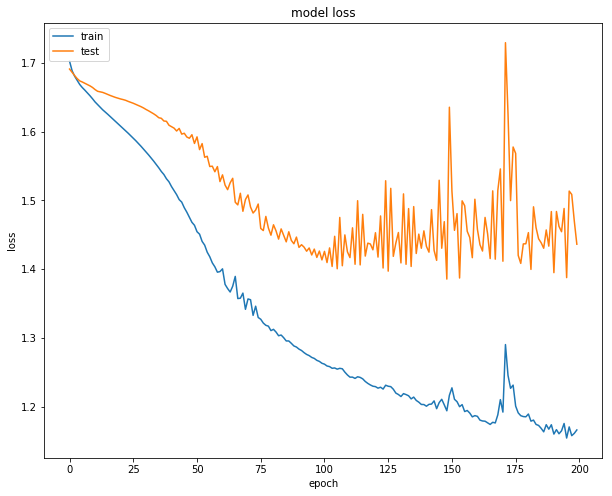
\includegraphics[width=0.45\textwidth]{LSTM_Loss_GD.png}
	\caption{Accuracy and loss v.s. number of epochs for the LSTM model on gesture data}
	\label{fig:learning_curve}
\end{figure}

Since the number of data after splitting is only 1K, there are some over-fitting problem when training this network. The validation accuracy is around $0.42$. Compared to TICC's accuracy $0.14$, it is already a lot more higher. The confusion matrix is shown in Fig. 6.

\begin{figure}[H]
	\centering
	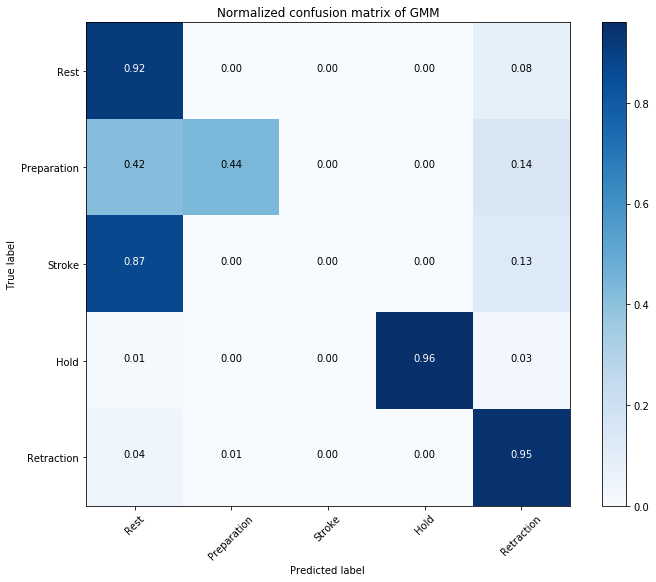
\includegraphics[width=0.45\textwidth]{LSTM_CFM_GD.png}
	\caption{Confusion matrix of prediction of LSTM on gesture data set}
	\label{fig:LSTM_CFM}
\end{figure}

Based on these facts, we can conclude that LSTM methods generally works better on sequences whose consisting sub-sequences are small. As analyzed in the previous section, the labels of gesture data changes frequently so that TICC fails to capture the small sub-sequences and LSTM on truncated sample sequences generally work.

However, things change when the switching between states become less frequent, when we compare LSTM and TICC on human activity data. We train a LSTM network with the same structure on 1K truncated human activity sequence of lenth 25, and the best validation accuracy is only around $0.45$.

\begin{figure}[H]
	\centering
	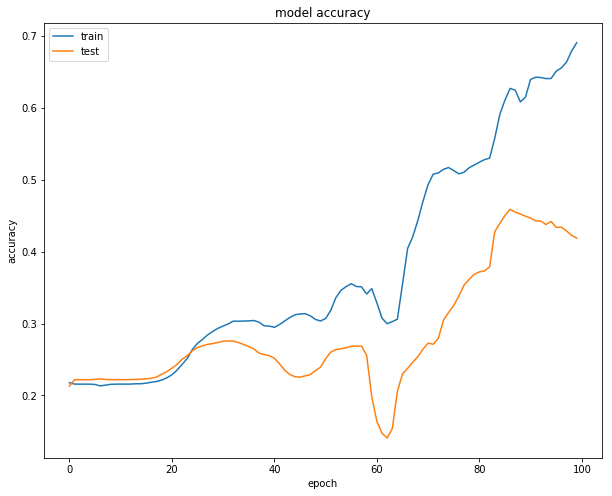
\includegraphics[width=0.45\textwidth]{LSTM_Accuracy_HAD.png}
	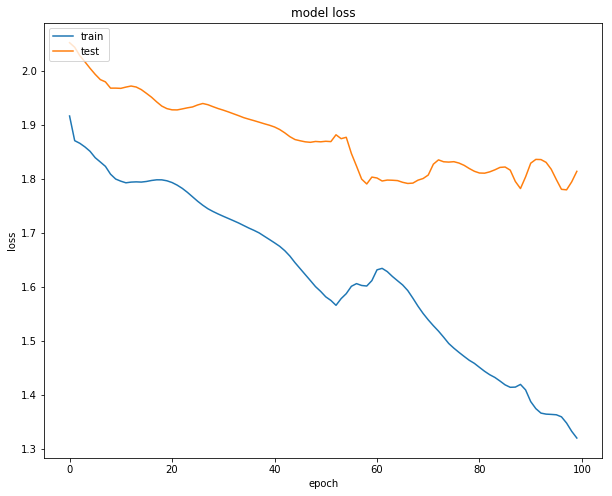
\includegraphics[width=0.45\textwidth]{LSTM_Loss_HAD.png}
	\caption{Accuracy and loss v.s. number of epochs for the LSTM model on human activity data}
	\label{fig:learning_curve2}
\end{figure}

Thus we can conclude that the TICC model is more capable to capture latent sub-sequence structure when the average length of them is enough long. Meanwhile, we have to split the full sequence before feeding into LSTM and this pre-processing step may already destroy may latent sub-sequence structure. The power of LSTM is thus greatly affected since the sequences feed in to it are not correctly aligned to each others. 

\section{Hyper-Parameter Tuning}
In this section, we examine the effect of different parameters to the accuracy and cluster property based on the empirical study on applying TICC model on Human Activities Dataset.

\subsection{Effects of the Hyper-Parameters}

\subsubsection{Smoothing Penalty:} This parameter determines the number of segment of a time series. When the smoothing penalty is higher, two small different contiguous clusters will merge to one cluster. As we can see in Fig. 8, smaller smoothing penalty yields more segments, with small strips in the time series. For a larger smoothing penalty, the amount of strips decreases (Fig. 8b) and eventually are smoothed to several pure large segments (Fig. 8c). This may reveal one limit of TICC algorithm in clustering frequently-changing time series.

\begin{figure}[H]
    \centering
    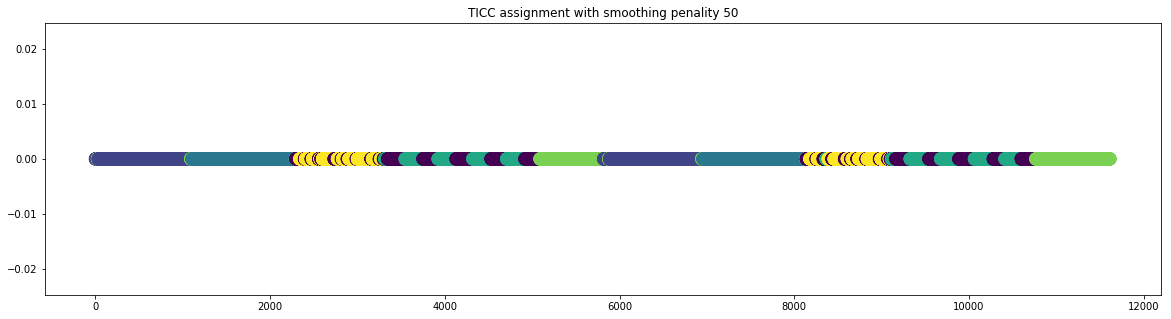
\includegraphics[width=.5\textwidth]{50Penalty.png}\hfill
    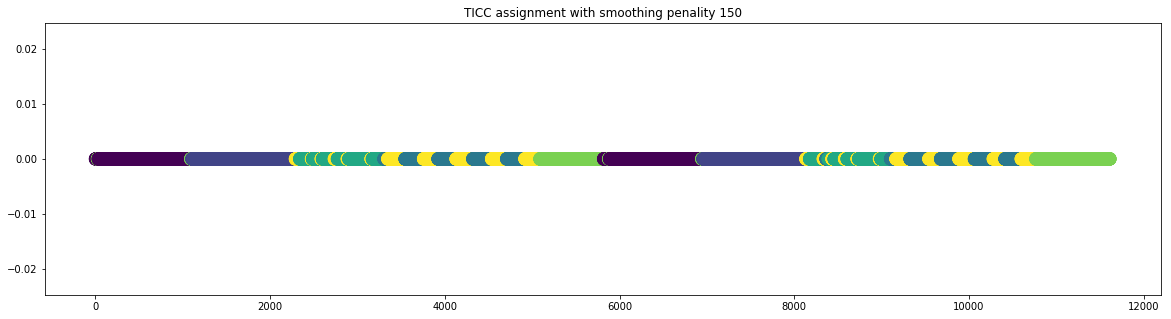
\includegraphics[width=.5\textwidth]{150Penalty.png}
    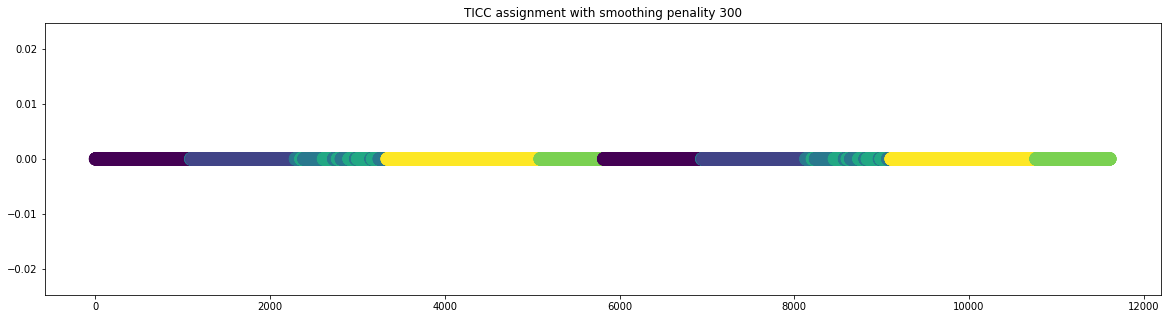
\includegraphics[width=.5\textwidth]{300Penalty.png}\hfill
    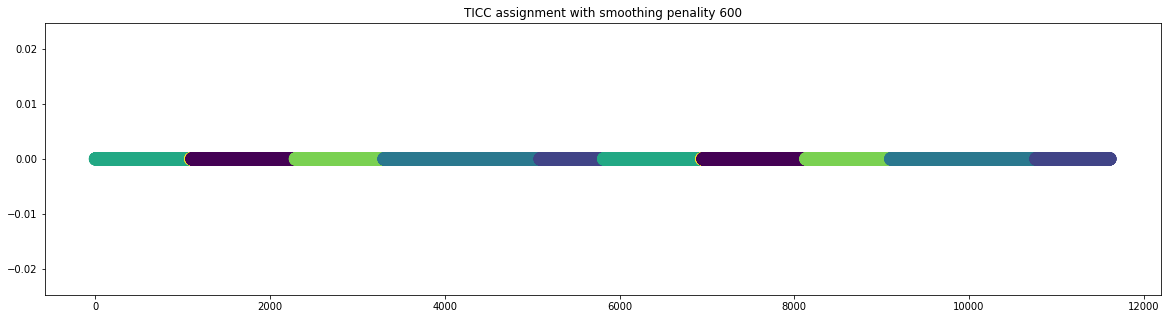
\includegraphics[width=.5\textwidth]{600Penalty.png}
    \caption{Human Activity Cluster assignment of smoothing penalty equals to (a) 50 (b) 150 (c) 300 (d) 600}
    \label{fig:penalty}
\end{figure}

\subsubsection{Regularization:} This parameter regularizes
the sparsity level of the MRF graph characterizing each cluster. Looking at the clustering assignment may not have immediate interpretation on the effect of changing the parameters (Fig. 9). 

\begin{figure}[H]
    \centering
    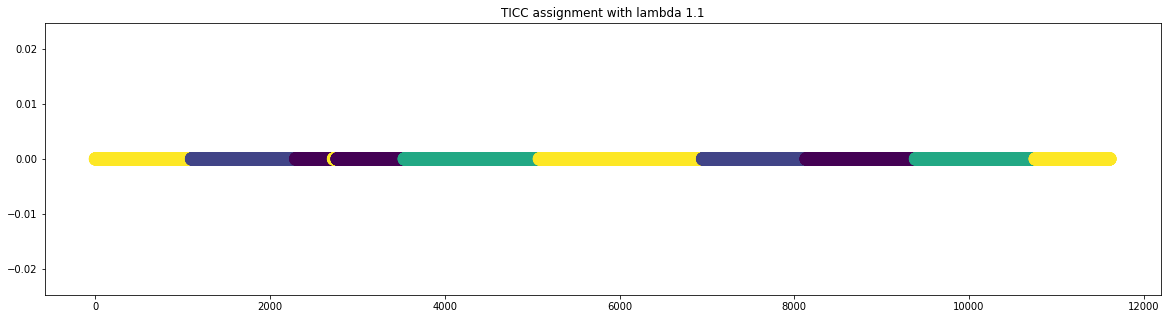
\includegraphics[width=.5\textwidth]{lambda1+1.png}\hfill
    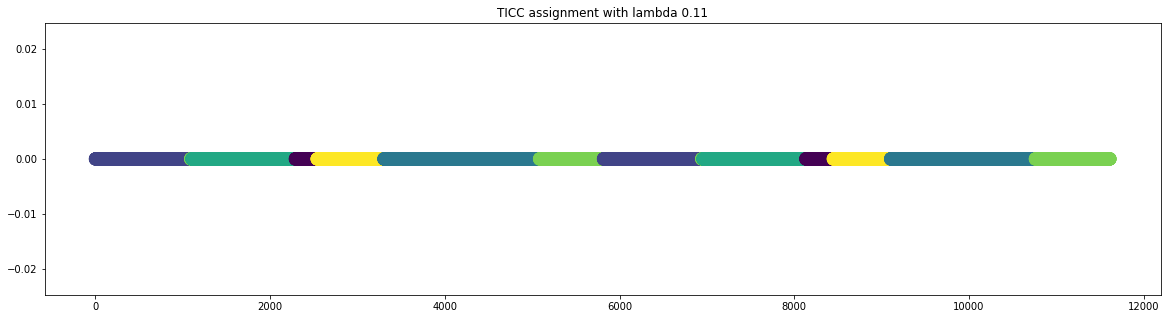
\includegraphics[width=.5\textwidth]{lambda0+11.png}
    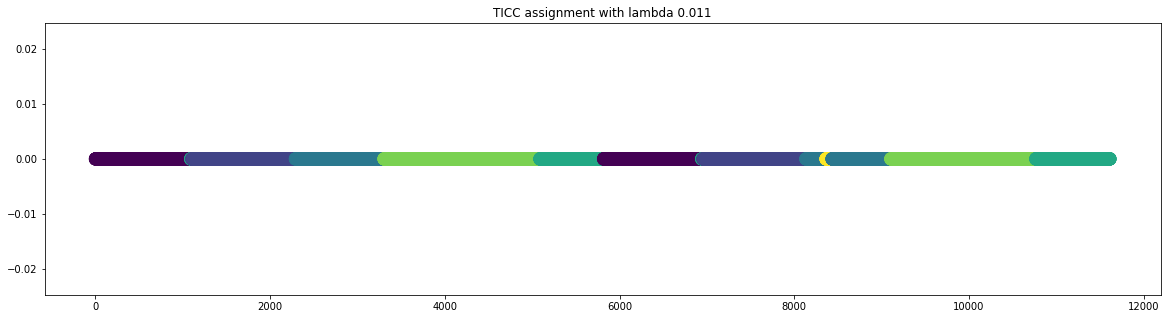
\includegraphics[width=.5\textwidth]{lambda+011.png}\hfill
    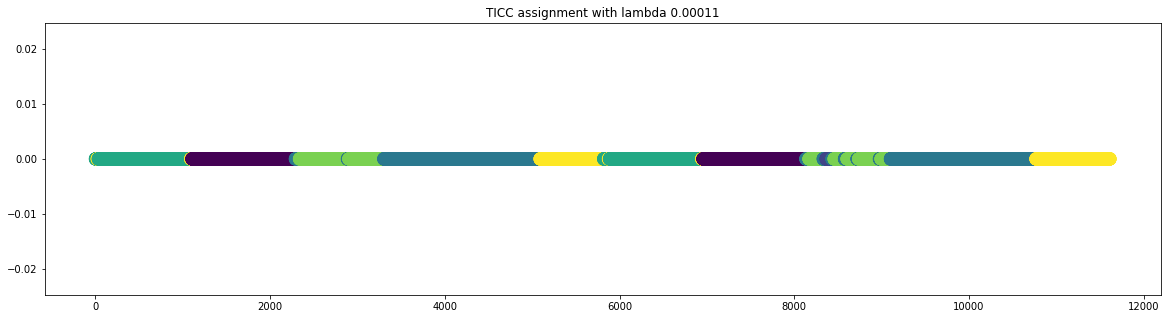
\includegraphics[width=.5\textwidth]{lambda0+00011.png}
    \caption{Human Activity Cluster assignment of regularization equals to (a) 1.1 (b) 0.11 (c) 0.011 (d) 0.00011}
    \label{fig:reg}
\end{figure}

Different clustering methods has its own representation of cluster, for example, KMeans can use mean of the data within that cluster, and GMM uses probability parameters. In TICC, each cluster is represented as a graph, called MRF. To observe the effect of regularizer parameter, we can observe the representation of each cluster. Fig. q0 shows the representation of the clusters when regularizer weight is set to 0.00011.

\begin{figure}[H]
    \centering
    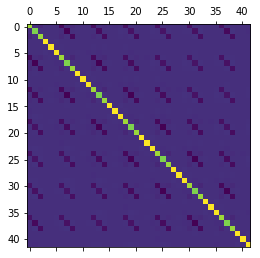
\includegraphics[width=.3\textwidth]{stand.png}\hfill
    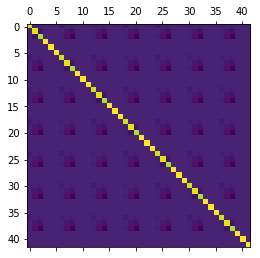
\includegraphics[width=.3\textwidth]{sit.png}\hfill
    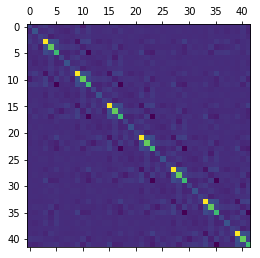
\includegraphics[width=.3\textwidth]{bike.png}
    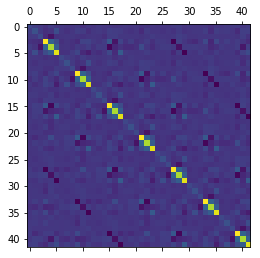
\includegraphics[width=.3\textwidth]{walk.png}\hfill
    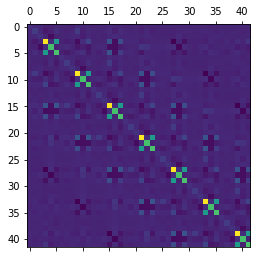
\includegraphics[width=.3\textwidth]{stairsup.png}\hfill
    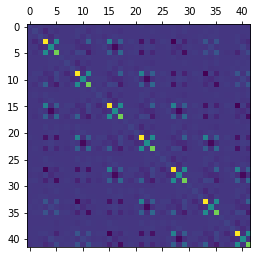
\includegraphics[width=.3\textwidth]{stairsdown.png}
    \caption{The graphical plot of the correlation network (MRF) with regularization 0.00011 of (a) Stand (b) Sit (c) Bike (d) Walk (e) Stairs Up (f) Stairs Down}
    \label{fig:mrf1}
\end{figure}

TICC represents Stand and Sit in similar graph similarly (Fig 10a, 10b). For Stairs Up and Stairs Down activities, they look also quite similar. (Fig 10e, 10f). For Biking (Fig. 10c), it looks closer to Stand and Sit than to stairs up and down; while Walking is vice versa. This is in fact coincide with human interpretation of the events, which is not hard to imagine that, walking movement is similar to that of walking up and down stairs, while the movement of standing and siting are more or less the same.

\begin{figure}[H]
    \centering
    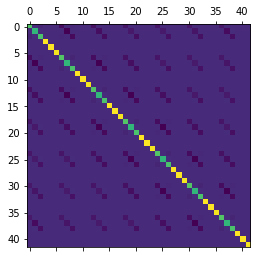
\includegraphics[width=.3\textwidth]{StandL.png}\hfill
    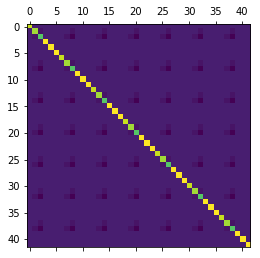
\includegraphics[width=.3\textwidth]{SitL.png}\hfill
    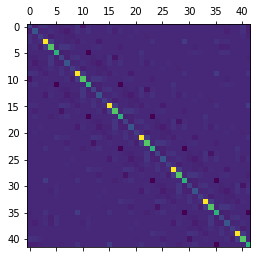
\includegraphics[width=.3\textwidth]{BikeL.png}
    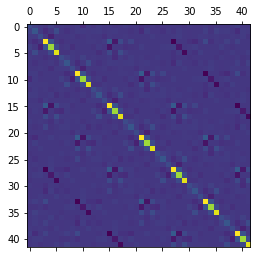
\includegraphics[width=.3\textwidth]{WalkL.png}\hfill
    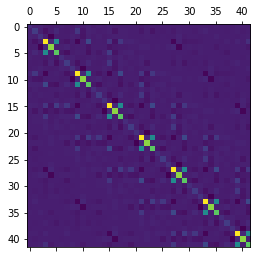
\includegraphics[width=.3\textwidth]{StairUpL.png}\hfill
    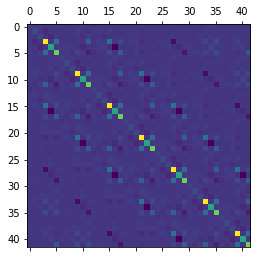
\includegraphics[width=.3\textwidth]{StairDownL.png}
    \caption{The graphical plot of the correlation network (MRF) with regularization 0.011 of (a) Stand (b) Sit (c) Bike (d) Walk (e) Stairs Up (f) Stairs Down}
    \label{fig:mrf2}
\end{figure}

When we carefully examine the cluster MRFs, the difference between with larger Fig. 10e and 11e is more observable. With larger regularization, the graph is less clear and the pattern are less sharp. The pattern of other plots from Fig. 11 is also slightly more blur than that of Fig. 10. This suggests that the more regularization leads to more general representation, possibly avoid over-fitting problem.

\subsubsection{Window Size:} This parameter controls the consideration of cross-time correlation, which means sensor reading at time t affect some sensor readings at time t + w, where w is the window size. A larger window size would reach a longer duration. As the window size increase, the shorter activities, that is the alternating stairs up and stairs down activity disappear and merge into one cluster. This is likely due to considering too long dependency between readings, causing local correlation to be diminished, thus fail to detect changes in shorter period activities. 

\begin{figure}[H]
    \centering
    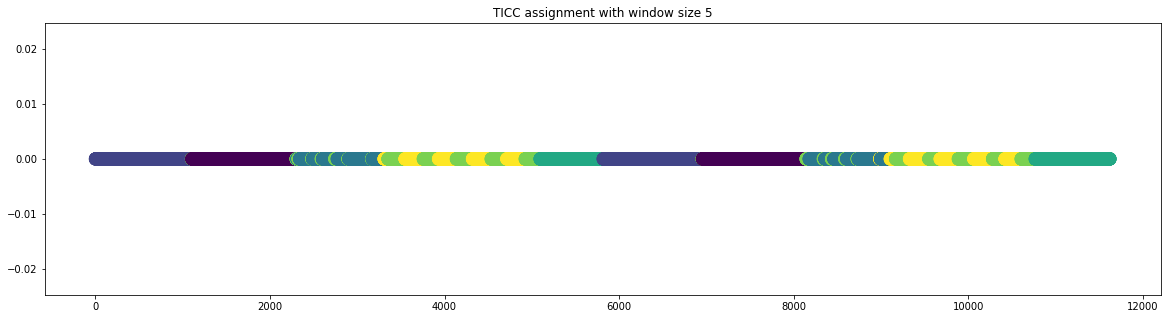
\includegraphics[width=.5\textwidth]{window5.png}\hfill
    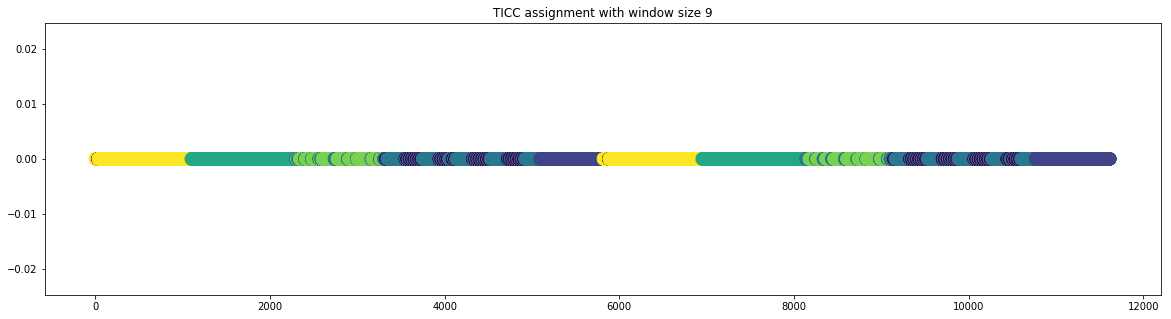
\includegraphics[width=.5\textwidth]{window9.png}
    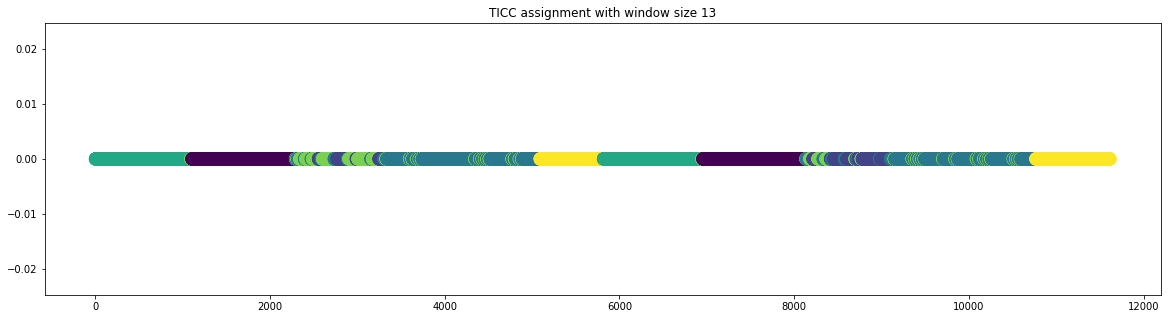
\includegraphics[width=.5\textwidth]{window13.png}\hfill
    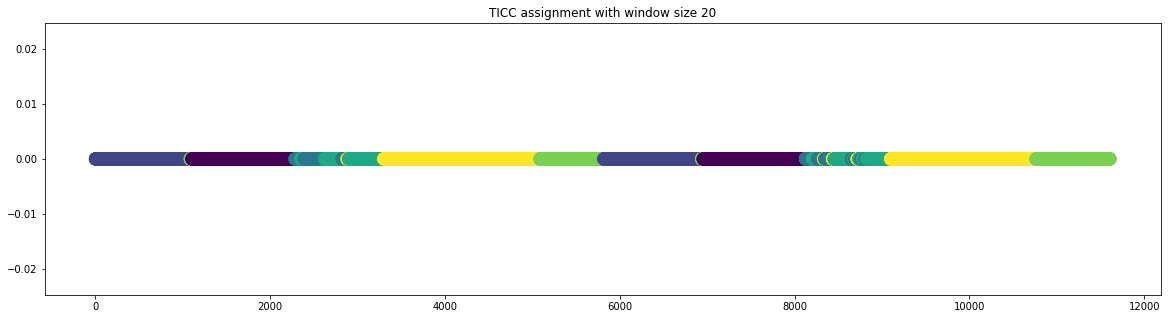
\includegraphics[width=.5\textwidth]{window20.png}
    \caption{Human Activity Cluster assignment of window size equals to (a) 5 (b) 9 (c) 13 (d) 20}
    \label{fig:window}
\end{figure}

\subsubsection{Dataset Size:}We also investigate TICC performance depending on the size of data. In data set of size 20K and 10K, it generates assignments with high accuracy up to 92\%, while KMeans and GMM generates 43\% and 58\% respectively. We notice that to achieve same accuracy as KMeans and GMM, TICC requires much less data, around 1600 data points, in this particular Human Activity Dataset.

\subsection{Choosing the Hyper-Parameters}
Based on the empirical results we obtained, we see how clustering characteristic changes with different parameters. In general, to cluster dataset with large segments (activities with long period of time), the larger window size and higher smoothing penalty could be employed. For more general solution, larger regularization parameter can be set.

\begin{figure}[H]
    \centering
    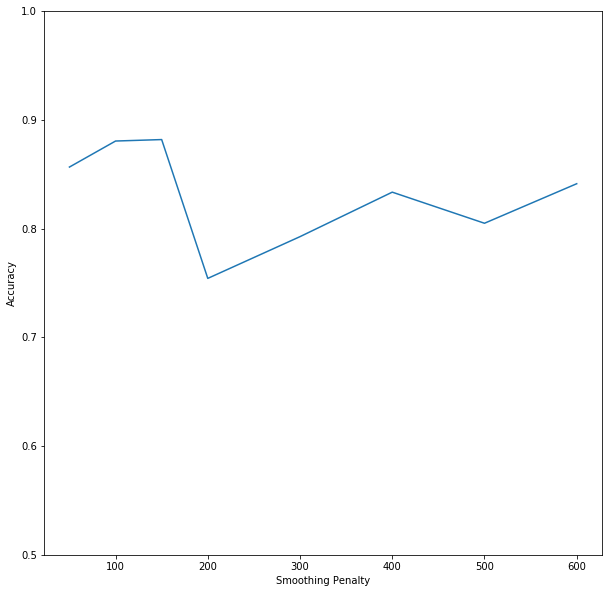
\includegraphics[width=.3\textwidth]{PenaltyLine.png}\hfill
    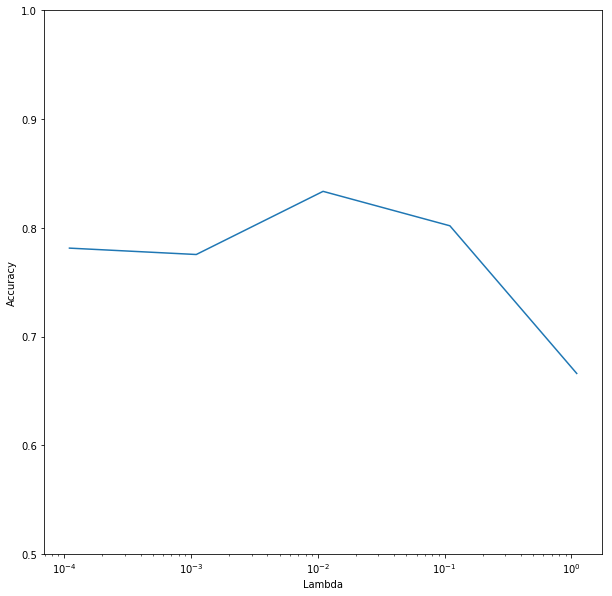
\includegraphics[width=.3\textwidth]{lambdaLine.png}\hfill
    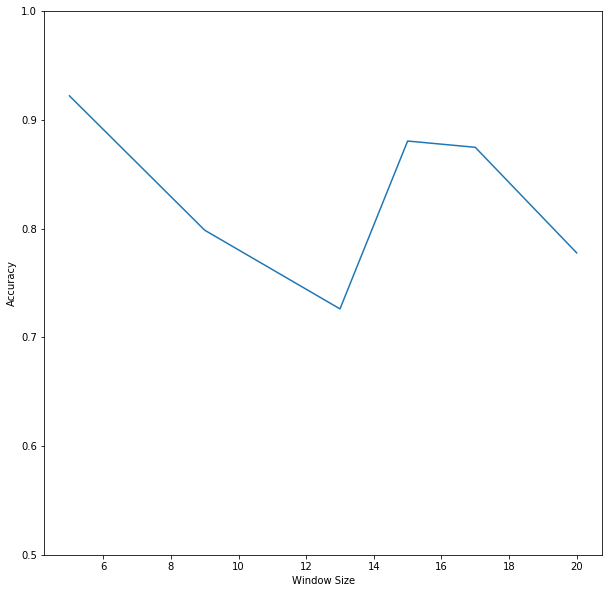
\includegraphics[width=.3\textwidth]{windowLine.png}
    \caption{Accuracy for different parameters values (a) smoothing penalty (b) regularization weight (c) window size}
    \label{fig:line}
\end{figure}

\section{Conclusions}


%
% ---- Bibliography ----
%

\bibliographystyle{splncs03}
\bibliography{Final}

\end{document}